\documentclass[10pt]{report}
\usepackage{amsmath}
\usepackage{hyperref}
\usepackage{graphicx}
\usepackage{color}
\title{Robotic Raditherepy}
\author{Rushabh Hathi}
\begin{document}
\maketitle
\chapter{Introduction}
The goal of the project is to plan a trajectory for a 7DOF robot in an environment where the targets are moving along with the obstacles. 
\\
Specifically, we are designing a robotic radiotherapy system which can automate the radiation dosage to the patients. The major feature of the system is to optimize the dosage such that the amount of radiation to the affected area(tumour) is maximum and to other organs is minimum. This goal is to be achieved in a dynamic environment where both the tumour and organs can move. 
\\
\\
This document provides details of the formulation of the problem that we just described. We convert this requirement into a technical specification.The next section provides details of the major issues that we need to address before actual implementation. Section \ref{assumptions} describes the assumptions we make. Then , we provide a basic formulation of the forward kinematics of the problem and also how we implement some of the assumptions. Section \ref{cost_function} provides the definition of cost function is provided with a detailed explanation. The document ends with a rationale about the cost function and assumptions.
\section{Issues}
This section provides details of the major issues that we intend to address while solving the aforementioned optimization problem. 
The major issues are:
\begin{enumerate}
\item How is the amount of dosage represented/calculated.
\item How is the cost of dosage defined.
%\item How is the cost of dosage calculated.
\item How to address the issue of moving targets and obstacles.
\item How to address issue of cumulative weights and tolerance levels.
\end{enumerate}
Most of the issues are concerned with how the different aspects of project requirements can be formalized in a mathematical specification.It will be seen in the remainder of this document that these challenges can be met by making proper assumptions and designing proper cost function for optimization.

\section{Assumptions}
\label{assumptions}
As mentioned above,to convert the requirements into a practically solvable problem and representing the system in terms of equations, we make certain assumptions. This section provides details on the assumptions we make regarding the system.
\\
\\
The fist and foremost point to consider is that the workspace( the space or volume where the radiation will be given) is continuous. This is an issue as the computation of any sort is difficult to carry out. Thus, for the ease of computation and without loss of generality, we discretize the work space.
The way this can achieved is using spheres to approximate the regions of the volume.The spheres can overlap with each other.
This is shown diagrammatically in figure \ref{fig_workspace}. 
\\
\\
\begin{figure}[h]
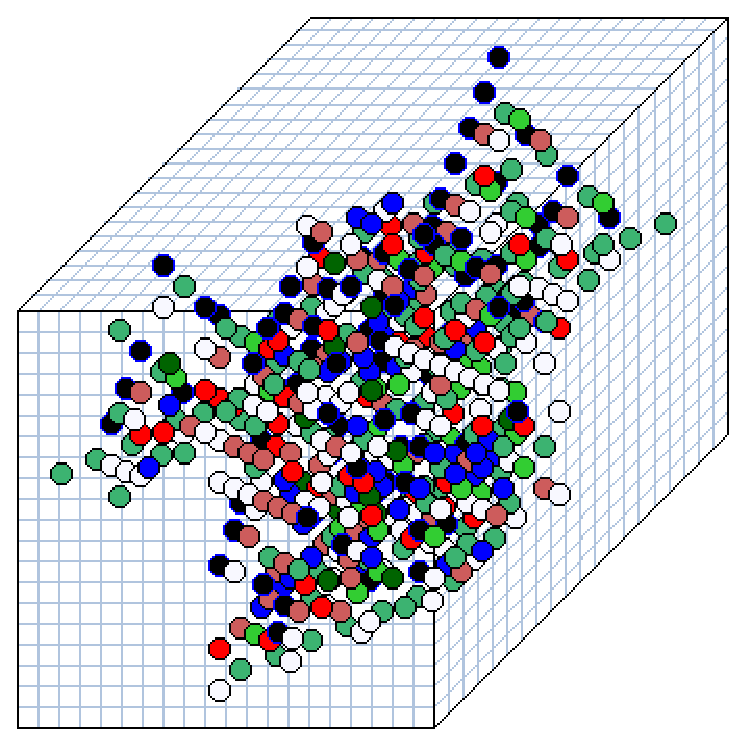
\includegraphics[scale=0.5]{resources/images/workspace.eps} 
\caption{Work space discretization}
\label{fig_workspace}
\end{figure}
As shown, the cube is the volume where the robotic arm can move. It can be approximated using various spheres which may overlap with each other. The collection of spheres will represent a region in the space.
As it will be seen in section \ref{cost_function} , such an approximation is advantageous as it makes the computation of the cost of dosage very simple.
\\
\\
We also make an assumption that the regions enveloped by the tumour and organs is known. This is an information which comes from the sensors and models but in this set-up we can assume to know it.
\\
\\
Referring to figure \ref{fig_patient}, the green sphere shows the region of the tumour which we want to target and the black spheres indicate the organs which ideally we want to avoid radiating. We assume that such a map is given with exact locations of tumorous regions and organs.
\begin{figure}
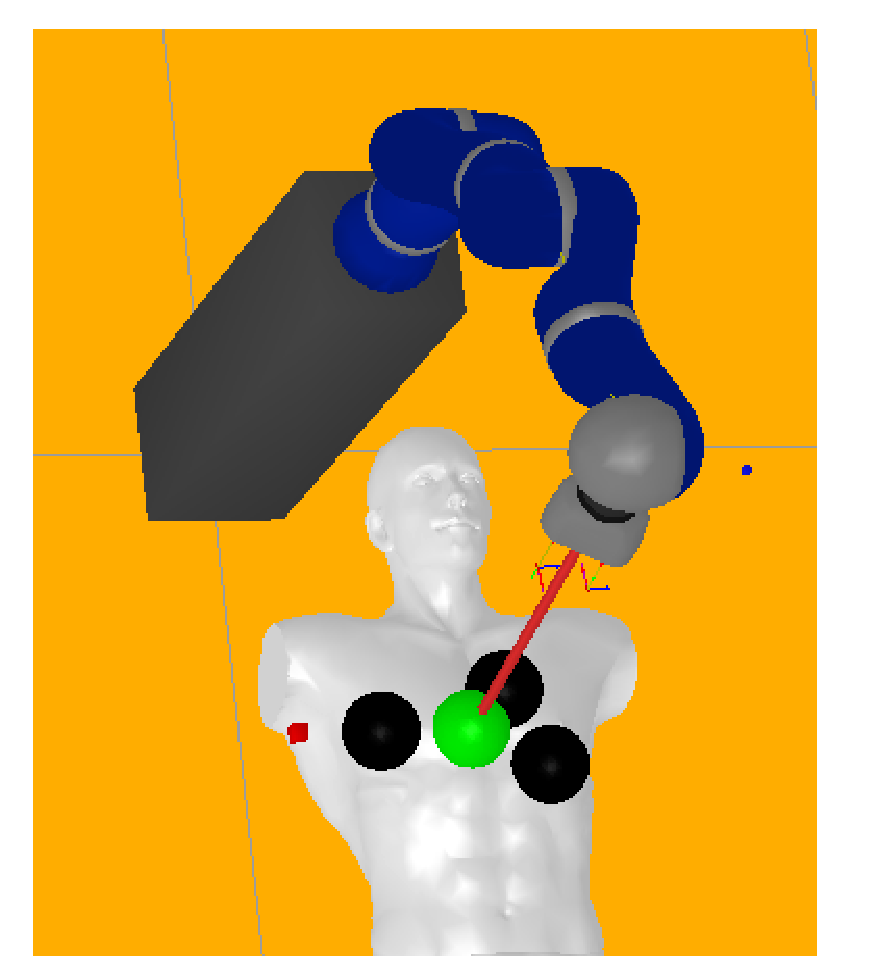
\includegraphics[scale=0.5]{resources/images/patient.eps} 
\caption{The deterministic volume of work space.}
\label{fig_patient}
\end{figure}
In modelling, we assume that the beam (ray) is an extension of the robotic arm. This is an important assumption as using this we can control the robot such that beam always passes through a desired point or region in the volume of workspace. With this assumption, this is trivial to achieve as will be seen below.
\\
\\
Another important assumption is that there is a parameter associated with each of the sphere in the workspace.This parameter is called "weight" and will be defined and used in section \ref{cost_function}.We will see that it is a very important part of the cost function and will help us to model the cumulative dosage cost as well as to manage dosage based on tolerance level. 
\\
\\
The amount of dosage is a complex challenge.It is not trivial to define or measure the amount of dosage. For the purpose of this project, we assume the amount of dosage is equal to the time of exposure. Thus, if the beam falls on a point for t seconds, we assume the amount of dosage to that point is t units.
\\
\\
We also assume for the purpose of this project that the tolerance levels of different regions is available to us.We can call this as "dose map" which gets updated with time.
\section{Basic Formulation}
This section shows the basic formulation of the problem with equations. It shows the structure and kinematic equations of the robotic arm and defines constraints on the robot. In this section, we also show how can we ensure that the beam always passes through the tumour.
\\
\\
Let us denote the vector of joint orientations as "q" and the end effector orientation as "y".We define a forward mapping from joint vector to end effector.
\begin{equation}
y=\phi(q)
\end{equation}
This also enables us to define the Jacobian:
\begin{eqnarray}
\dot{y}=J(q) \dot{\phi(q)} \\
J(q)= \frac{\partial \phi(q)}{ \partial q}
\end{eqnarray}
\\
\\
As mentioned in section \ref{assumptions}, we model the ray as an extension of the robotic arm. Once this is done, we can define a constraint to ensure that the ray always passes through the tumour.This is shown.
\\
Suppose the position vector or the tumour is known as 'p'.
The constraint would be 
\begin{equation}
C(q,p)=0
\end{equation}
Its important to note here that 'p' is an external parameter that we either know or obtain from an external source(sensor data). The idea of this constraint is that the joint vector should be such that a line is defined by the end effector and the tumour.(Thus all joint vector which orient the end effector such that no line is defined are discarded).
This would force the ray to pass through the tumour(target region).
\\
\\
Once we have such basic formulation , we can proceed to define the cost function.
\subsection{Cost Function}
\label{cost_function}

This section provides details of the design of cost function. This is one of the most important part of the project as this will be used (minimized) for optimization. It is important for the cost function to reflect the objectives that a good trajectory should have. It will be shown that using the cost function, we can capture many aspects of the system and thus achieve the desired trajectory.
\\
\\
We know that the workspace has been discretized and is represented by a set of spheres. We also have defined the ray as a line between end effector and the tumour. Using this knowledge , we formulate the cost function.
\\
Define a line from the end effector position(y) to the target region( a point in tumour), which is the ray.
\\
Denote the line as 'l'

Once the beam is defined, the cost of the dose can be formulated as the sum of distances of all the sphere centers from the beam.

The form of the cost function will be:
\begin{equation}
J(t)=\sum_{i=1}^{N} (C_i(t) \cdot l )w_i(t,h)
\end{equation}
${C_i}$ are the centers of the spheres,we have defined. Dependence of ${C_i}$  on time is essential as using this , we can model the ,movement of the tumour and the obstacles in the region with time.
${w_i}$ are the weight parameter associated with the spheres."h" is the history of dosage which would effect the weight of the point.This is a very important aspect of the cost function. W(t,h) is the function which determined the weights of each sphere. This weight is determined based on the amount of dosage given to the point till now as well as the tolerance level. Thus, if a region has already reached its tolerance level , the weights would be higher making the overall cost very high. Thus, using a single function, we can model cumulative dosage and tolerance of the regions.
\\
\\
This can be well understood in terms of a simple diagram.Referring to figure \ref{fig_cost}, we denote the region of organs by orange spheres and of tumour by green spheres.The cost is now the weighted sum of the perpendicular distance from each sphere to the ray(red line). This also helps us calculate the volume of region affected by a single beam if we keep a threshold. The weight would change based on total dosage given till now. 
\begin{figure}
\includegraphics[scale=0.4]{resources/images/cost.png}[h]
\caption{Calculation of cost function.}
\label{fig_cost}
\end{figure}
In terms of distance function d it can be:
\begin{equation}motivation
J(t)=\sum_{i=1}^{N} (distance(C_i(t),l))w_i(t,h)
\end{equation}

\subsection{Rationale}
The rationale behind such a cost function are listed below:
\begin{enumerate}
\item The weights of OARs can be negative initially to achieve the goal of beam being away from OAR.
\item The dependence of weights on time and history would capture the effects of cumulative dosage and tolerance levels of regions.
\item The dependence of points on time is important as it can capture the fact that the points are moving and thus the cost function for exactly the same orientation of the end effector would be different.
\item It does not represent the traditional theory of "further the better" as we might hit an important area of the tumour by a beam passing very closely through an OAR which is beneficial and can be achieved by tweaking the weights in the cost function.
\end{enumerate}
\end{document}



